\documentclass{article}
\usepackage{multicol}
\usepackage{graphicx}
\usepackage{xcolor}
\definecolor{keyword}{rgb}{0.3568627451, 0.7372549020, 0.6431372549}
\definecolor{comment}{rgb}{0.5411764706, 0.7490196078, 0.3450980392}
\definecolor{string}{rgb}{0.9,0.4,0}
\definecolor{function}{rgb}{0.5,0.5,0.1}
\usepackage{listings}
\lstset{
    basicstyle=\small\ttfamily,
    breaklines=true,
    frame=single,
    rulecolor = \color{gray},
    numbers=left,
    numbersep=5pt,
    numberstyle=\tiny,
    showstringspaces=false,
    tabsize=4,
    keywordstyle=\color{keyword},
    commentstyle=\color{comment},
    stringstyle=\color{string},
}
\usepackage{hyperref}
\hypersetup{
    colorlinks=true,
    urlcolor=cyan,
}
\usepackage{makecell}
\usepackage[a4paper, margin=1in]{geometry}
\usepackage{float}

\title{Cloud Computing - Project Report \\ \small{Totoro Group}}
\author{
    Zahra Omrani \\ z.omrani@studenti.unipi.it \and 
    Paolo Palumbo \\ p.palumbo3@studenti.unipi.it \and
    Ettore Ricci \\ e.ricci32@studenti.unipi.it}

\begin{document}
\maketitle
\begin{center}
    \scriptsize
    \href{https://github.com/Etto48/CloudComputingProject}{https://github.com/Etto48/CloudComputingProject}
\end{center}

\begin{abstract}
    This report presents the development and performance evaluation of a Java-based application 
    designed to count letter frequencies in large datasets using the Hadoop framework. 
    To provide a comprehensive analysis, we also implemented and tested non-distributed 
    applications in Python and Rust for comparison.
    The results show that for the sizes of the datasets considered, Java and Python execution 
    times are comparable, while Rust is significantly faster. 
    Both Python and Rust applications used significantly less memory than the Java application.
\end{abstract}
\begin{multicols}{2}
\section{Introduction}
    Our project for the Cloud Computing course consists of developing a Java application to count
    the frequency of letters in a large dataset using the Hadoop framework.
    The main objective of the project is to analyze and compare the performance of the application
    with different configurations and input sizes and also to compare it with non-distributed
    implementations in Python and Rust.
\section{Mapreduce}
    MapReduce is a programming model for processing large data sets. 
    Users specify a map function that processes a key/value pair to generate a set
    of intermediate key/value pairs, and a reduce function that merges all intermediate values
    associated with the same intermediate key.
    For our application we needed two subsequent MapReduce jobs: the first one to count the occurrences
    of each letter in the input text and the second one to calculate the frequency of each letter.
    \subsection{Job 1: Counting letters}
        \subsubsection{Mapper}
            For testing purposes, we created two different mappers: one with an in-mapper combiner and one 
            without.
            For the combiner (when enabled), we used the same code as the reducer.
            \begin{itemize}
                \item \textbf{Mapper with in-mapper combiner}:
                This mapper stores the letter counts in a vector and emits them in the cleanup method.
                At the end of the cleanup method, the mapper increments a job counter with the number of emitted 
                letters.
                (Listing \ref{lst:java_mapper})
                \item \textbf{Mapper without in-mapper combiner}: 
                This mapper emits the letter counts (with value 1) for each letter in the map method.
                At the end of the map method, the mapper increments a job counter with the number of emitted
                letters.
                (Listing \ref{lst:java_mapper_no_combiner})
            \end{itemize}
        \subsubsection{Reducer}
            The reducer receives the letter counts from the mappers and sums them up.
            (Listing \ref{lst:java_reducer})
    \subsection{Job 2: Calculating frequencies}
        The results of the first job are saved in a temporary file and used as input for the second job.
        The counter obtained from the first job is stored in a configuration variable that is passed to the 
        reducer (only one is needed because the number of different letters is small).
        For this job we do not need a combiner so it's always disabled.
        \subsubsection{Mapper}
            We used an identity mapper that emits the letter counts as they are.
        \subsubsection{Reducer}
            The reducer receives the letter counts from the mappers and calculates the frequency of each letter
            using the total count that was previously stored in a configuration variable.
            (Listing \ref{lst:java_reducer_frequency})
\section{Dataset}
    We used three different datasets:
    \begin{itemize}
        \item \textbf{english.txt}: A 1.2GB text file containing text from the books on \href{https://www.gutenberg.org/}{Gutenberg project}.
        \item \textbf{italian.txt}: A 1.3GB text file from the \href{https://www.corpusitaliano.it/}{PAISÀ corpus}\cite{lyding-etal-2014-paisa}.
        \item \textbf{spanish.txt}: A 130MB text file from the \href{https://wortschatz.uni-leipzig.de/en/download/Spanish}{Leipzig Corpora Collection}\cite{Eckart2013}.
    \end{itemize}
    We also created 11 files of increasing size (from 100MB to 1.1GB with 100MB steps) to test the performance
    of the application with different input sizes. These files are called \textbf{part\_$X$MB.txt} and 
    contain the first $X$MBs of the \textbf{english.txt} file. 
\section{Experiments}
    We wrote our program in a way that allows us to configure it for the different tests with 
    command line arguments:
    \begin{itemize}
        \item \textbf{$-i|--input$}: Input file path inside the HDFS.
        \item \textbf{$-r|--reducers$}: Number of reducers to use in the first job.
        \item \textbf{$-n|--no-combiner$}: Disable the combiner in the first job.
        \item \textbf{$-m|--no-in-mapper-combiner$}: Disable the in-mapper combiner in the first job.
        \item \textbf{$-o|--output$}: Output directory path inside the HDFS, 
        by default it's set to \textbf{output}.
        \item \textbf{$-t|--tmp$}: Temporary directory path inside the HDFS,
        by default it's set to \textbf{tmp}.
    \end{itemize}
    We carried out 21 tests with the configurations shown in 
    Table \ref{tab:general_tests} and Table \ref{tab:input_split_tests}.
    Originally we ran tests 7, 8 and 9 with 4 reducers, but test 9 could never complete because of a 
    Shuffle Error caused by a Java Heap Space error (Out Of Memory Error). Because of this, 
    we decided to run these tests again with 3 reducers.
    Only the 3 reducers configuration will be shown in the results.
    We also ran the Python and Rust applications with the same input file (english.txt).
    We tested two slightly different versions of the Python and Rust applications: one that reads the
    input file in an asynchronous way, discarding the parts of the file that have already been processed (file streaming),
    and one that first reads the whole file into memory and then processes it.
    \begin{table}[H]
        \centering
        \begin{tabular}{|c|l|}
            \hline
            Test ID & Arguments \\
            \hline
            0 & \makecell[l]{-i english.txt \\ -r 1} \\        
            \hline
            1 & \makecell[l]{-i english.txt \\ -r 2} \\        
            \hline
            2 & \makecell[l]{-i english.txt \\ -r 4} \\        
            \hline
            3 & \makecell[l]{-i english.txt \\ -r 8} \\        
            \hline
            4 & \makecell[l]{-i english.txt \\ -r 1 \\ --no-combiner} \\        
            \hline
            5 & \makecell[l]{-i english.txt \\ -r 1 \\ --no-in-mapper-combiner} \\        
            \hline
            6 & \makecell[l]{-i english.txt \\ -r 1 \\ --no-in-mapper-combiner \\ --no-combiner} \\        
            \hline
            7 & \makecell[l]{-i english.txt \\ -r 3 \\ --no-combiner} \\        
            \hline
            8 & \makecell[l]{-i english.txt \\ -r 3 \\ --no-in-mapper-combiner} \\        
            \hline
            9 & \makecell[l]{-i english.txt \\ -r 3 \\ --no-in-mapper-combiner \\ --no-combiner} \\        
            \hline
        \end{tabular}
        \caption{General tests}
        \label{tab:general_tests}
    \end{table}
    \begin{table}[H]
        \centering
        \begin{tabular}{|c|l|}
            \hline
            Test ID & Arguments \\
            \hline
            10 & \makecell[l]{-i part\_100MB.txt \\ -r 1} \\  
            \hline      
            11 & \makecell[l]{-i part\_200MB.txt \\ -r 1} \\  
            \hline      
            12 & \makecell[l]{-i part\_300MB.txt \\ -r 1} \\        
            \hline
            13 & \makecell[l]{-i part\_400MB.txt \\ -r 1} \\        
            \hline
            14 & \makecell[l]{-i part\_500MB.txt \\ -r 1} \\        
            \hline
            15 & \makecell[l]{-i part\_600MB.txt \\ -r 1} \\        
            \hline
            16 & \makecell[l]{-i part\_700MB.txt \\ -r 1} \\        
            \hline
            17 & \makecell[l]{-i part\_800MB.txt \\ -r 1} \\        
            \hline
            18 & \makecell[l]{-i part\_900MB.txt \\ -r 1} \\        
            \hline
            19 & \makecell[l]{-i part\_1000MB.txt \\ -r 1} \\        
            \hline
            20 & \makecell[l]{-i part\_1100MB.txt \\ -r 1} \\            
            \hline
        \end{tabular}
        \caption{Input split tests}
        \label{tab:input_split_tests}
    \end{table}
    \subsection{Equipment}
        The tests were carried out on 3 identical virtual machines, each one with the following specifications:
        \begin{itemize}
            \item \textbf{CPU}: 1 core (2 logical cores) of an Intel(R) Xeon(R) Silver 4208 CPU @ 2.10GHz
            \item \textbf{RAM}: 6.8GB
            \item \textbf{Disk}: 40GB
            \item \textbf{OS}: Ubuntu 22.04.4 LTS
        \end{itemize}
        The Java application used the whole equipment, while the Python and Rust applications used only one 
        logical core on one machine.
\section{Results}
    The results of the tests on the Java application are shown in Figure \ref{fig:tests_graph}.
    The memory usage over time of the Python and Rust applications is shown in Figure \ref{fig:baseline}.
    The frequencies of the letters calculated by the application are shown in 
    Figure \ref{fig:en_freq} for English, Figure \ref{fig:it_freq} for Italian and 
    Figure \ref{fig:es_freq} for Spanish.
    \begin{figure}[H]
        \centering
        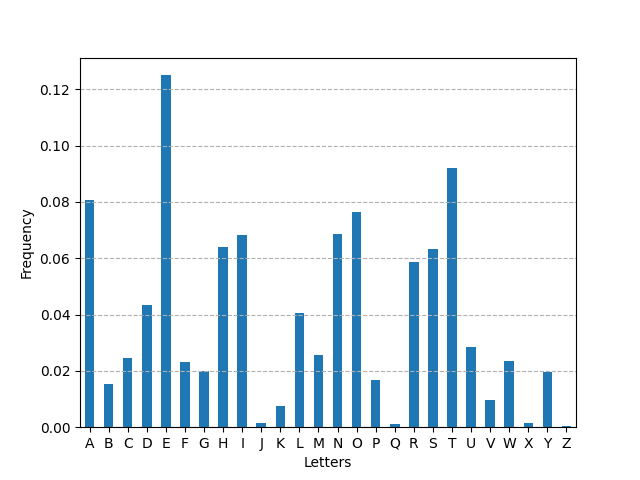
\includegraphics[width=0.48\textwidth]{figures/en.png}
        \caption{English letter frequency}
        \label{fig:en_freq}
    \end{figure}
    \begin{figure}[H]
        \centering
        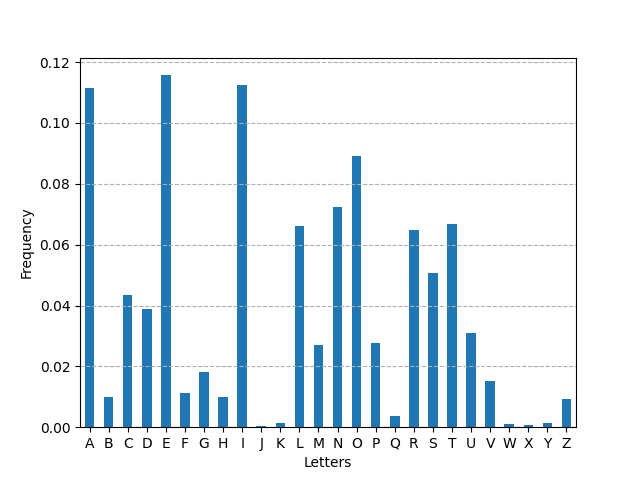
\includegraphics[width=0.48\textwidth]{figures/it.png}
        \caption{Italian letter frequency}
        \label{fig:it_freq}
    \end{figure}
    \begin{figure}[H]
        \centering
        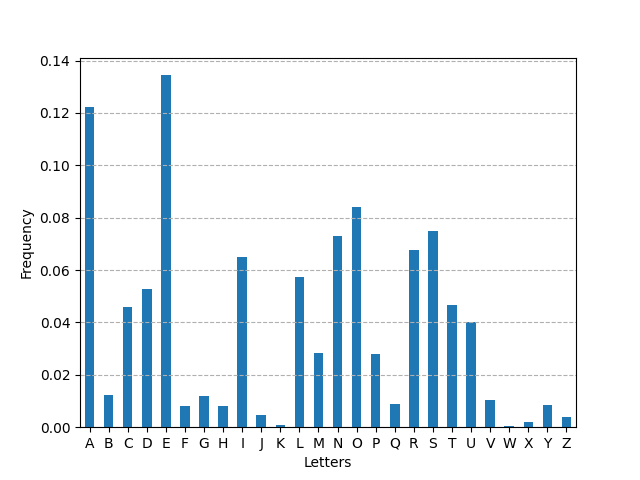
\includegraphics[width=0.48\textwidth]{figures/es.png}
        \caption{Spanish letter frequency}
        \label{fig:es_freq}
    \end{figure}
    \subsection{Java}
        \subsubsection{Execution time}
            From Figure \ref{fig:tests_graph} (Execution time) we can see that the execution time of the
            Java application with the complete dataset as imput (Tests $[0,9]$) has a minimum value of 76s and
            a maximum value of 893s.
            Execution time increases significantly when the in-mapper combiner is not used (Tests ${5,6,8,9}$)
            and increases further when the combiners are also disabled (Tests ${6,9}$).
            More reducers lead to a slight increase in execution time when using the in-mapper combiner 
            (Tests ${0,1,2,3}$). Execution time of Test 9 is smaller than the one of Test 6 because the
            higher number of reducers helps with the processing speed of the big amount of data produced 
            by the mappers without in-mapper combiners nor combiners.
            In all other cases, the overhead of more reducers is not compensated by the speedup in processing.
            We suppose that a big factor in this overhead is the memory usage increase due to the necessity of
            a shuffle phase.
            On the other hand, we can see from Tests $[10,20]$ that the execution time is almost constant
            (~56s) until the input size reaches 600MB (Test 15), after which it starts to increase linearly
            up to 76s for the 1.2GB input file (Test 0).
        \subsubsection{Memory usage}
            We can see from the top two graphs in Figure \ref{fig:tests_graph} that the memory usage of the Java
            application is very high, reaching 61.3GB of virtual memory in Test 3.
            The memory usage increases with the number of reducers. 
            The absence of the in-mapper combiner and the combiner does not significantly affect the 
            total virtual memory usage. On the other hand, it significantly increases the virtual memory 
            usage of the reducers. 
            We think that this is due to the fact the most of the memory used by the mappers is released
            before the reducers start.
            We also see that the total memory usage scales linearly with the input size: with a minimum of
            7.2GB for the 100MB input file (Test 10) and a maximum of 36GB for the 1.2GB input file (Test 0).
            When we used 1 reducer, the memory usage of the second job was negligible compared to the first job.
            With more reducers, we had more input files for the second job, which increased the linearly
            the memory usage of the second job, up to 32.4GB for 8 reducers (Test 3).
    \subsection{Python}
        The Python application completed after 293s using file streaming and 298s without it, 
        taking approximately 4 times more than the Java application (Test 0).
        The memory usage is of 0.27GB with file streaming and 2.65GB without it, using up to 
        133 times less memory than the Java application (Test 0).
    \subsection{Rust}
        The Rust application completed after 24s using file streaming and 19s without it, taking
        3 to 4 times less than the Java application (Test 0).
        The memory usage is of 0.0075GB with file streaming and 4.26GB without it, using up to
        4800 times less memory than the Java application (Test 0).
        These results show the efficiency of Rust in terms of both execution time and memory usage and
        the huge overhead of an interpreted language plus the Hadoop framework.

\end{multicols}
\begin{figure}[H]
    \centering
    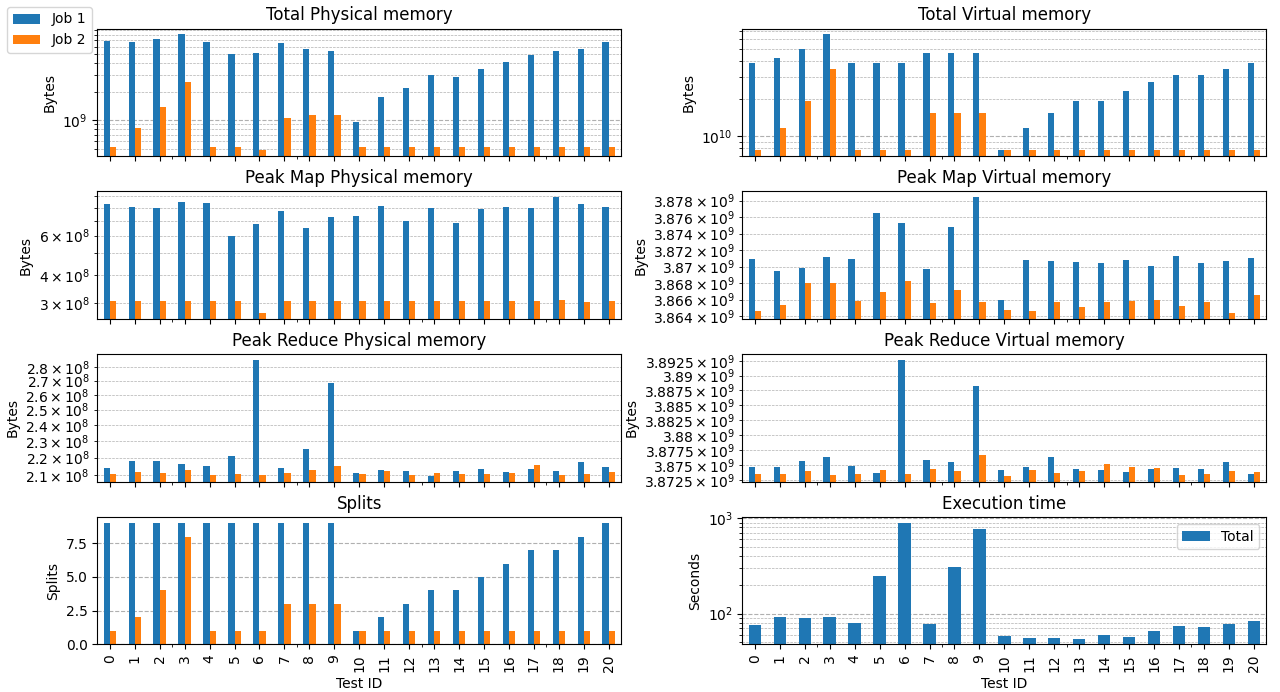
\includegraphics[width=1\textwidth]{figures/experiments.png}
    \caption{Tests results, the x-axis represents the test ID.}
    \label{fig:tests_graph}
\end{figure}
\begin{figure}[H]
    \centering
    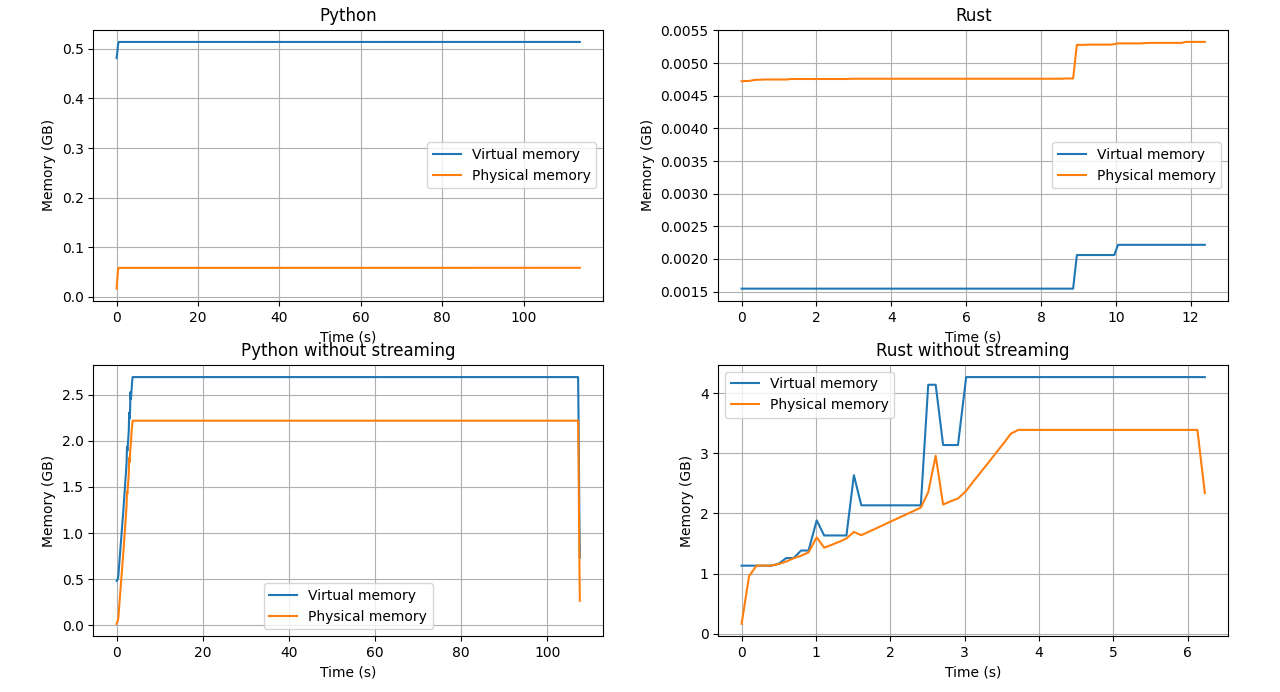
\includegraphics[width=1\textwidth]{figures/baseline.png}
    \caption{Python and Rust memory usage over time, with and without file streaming.}
    \label{fig:baseline}
\end{figure}
\begin{multicols}{2}

\section{Conclusions}
\end{multicols}
\section{Listings}
\lstinputlisting[
    language=Java, 
    caption={Mapper with in-mapper combiner},
    label={lst:java_mapper}
]{../letterfreq/src/main/java/it/unipi/Mapper.java}
\lstinputlisting[
    language=Java,
    caption={Mapper without in-mapper combiner},
    label={lst:java_mapper_no_combiner}
]{../letterfreq/src/main/java/it/unipi/MapperNoCombiner.java}
\lstinputlisting[
    language=Java,
    caption={Reducer},
    label={lst:java_reducer}
]{../letterfreq/src/main/java/it/unipi/Reducer.java}
\lstinputlisting[
    language=Java,
    caption={ReducerFrequency class, used to calculate the frequency of each letter},
    label={lst:java_reducer_frequency}
]{../letterfreq/src/main/java/it/unipi/ReducerFrequency.java}
\lstinputlisting[
    language=Java,
    caption={Char class, used as a custom key},
    label={lst:java_char}
]{../letterfreq/src/main/java/it/unipi/Char.java}

\bibliographystyle{IEEETran}
\bibliography{references.bib}
\end{document}